%!TEX root = ../thesis.tex
%*******************************************************************************
%****************************** Second Chapter *********************************
%*******************************************************************************

\chapter{The LHC}
\graphicspath{{2_Background/Figs/}}

This chapter provides the background of the project, with a focus on the MightyPix sensor, which is designed for use in the Mighty Tracker (MT) sub-detector of the LHCb experiment at the LHC. It introduces the LHC, the LHCb experiment, and the MT system to establish the motivation and application of MightyPix.


%********************************** %First Section  **************************************
\section{The Large Hadron Collider} 
\label{section2.1}
% Broad context of the LHC
The Large Hadron Collider (LHC) is by far the most powerful particle accelerator in the world\cite{CERNbrochure}. Constructed between 1998 and 2008, it is located 100 metres underground beneath the France–Switzerland border near Geneva. The LHC collides protons at a maximum collision energy of 13TeV, enabling exploration of a broad range of particle physics phenomena, including the study of supersymmetry, the matter-antimatter imbalance, dark matter and dark energy. It also facilitates heavy-ion collisions, providing a platform for investigating the quark-gluon plasma.

%, in the tunnel that previously housed the Large Electron-Positron Collider (LEP). LEP operated for 11 years and had achieved significant results, but its maximum collision energy (209MeV) was insufficient to probe highly suppressed processes. Instead, the LHC collides protons at a maximum collision energy of 13TeV, enabling exploration of a broader range of flavour physics phenomena. These include the study of supersymmetry, the matter-antimatter imbalance, dark matter and dark energy, etc. The LHC also facilitates heavy-ion collisions, providing a platform for investigating the quark-gluon plasma.

%The circular track of LHC is approximately 27 kilometres in circumference, where two beams of protons or ions travel in opposite directions, and collide at four interaction points. Before entering the circular track, the 40MHz proton beam is accelerated in a series of pre-accelerators. Firstly, in a linear accelerator (LINAC2), the protons are accelerated to 50MeV, then to 1.4GeV in the Proton Synchrotron booster. According to the need of the experiments, protons can be further boosted in Proton Synchrotron and Super Proton Synchrotron to 450GeV. The particles then fill the LHC in four minutes, and accelerate around the LHC in two beam pipelines.


%General information for HL-LHC upgrade
At the moment, the precision of the measurements at the LHC is limited by statistics. In other words, the accuracy is limited by finite data size, rather than instrumental limitations or systematic uncertainties. A proportional increase in data size can be achieved either by extending correspondingly the runtime of the experiment, or by increasing the luminosity of the beam. The luminosity measures the amount of particles passing through a given area per unit time in the beam - higher luminosity, more potential particle collisions. 

The High-Luminosity Large Hadron Collider project (HL-LHC) plans to increase the working luminosity to $5 \times 10^{34} cm^{-2} s^{-1}$ (about 5 times the current value), with annual data output of $250 fb^{-1}$ and $3000 fb^{-1}$ in 12 years after the upgrade\cite{HLLHC}. This would improve the performance of the current collider, exploiting its physics potential until the end of its life span\cite{CERNbrochure}.

High luminosity beam puts forward challenges for the detectors at the LHC. Larger number of proton-proton collision per bunch crossing\footnote{At the LHC, particles are accelerated in groups known as "bunches", with a time spacing of 25ns between successive bunches\cite{HLLHC}. A bunch crossing occurs when two bunches (one from each beam) pass through each other at an interaction point, and particle collisions can happen.} leads to a corresponding increase in the number of primary vertices\footnote{In one bunch crossing, multiple collisions can occur - between the protons, the products of pp collisions, etc. The protons are called the primary particles, as they start the collision event. A primary vertex is where the primary particles collide - it marks the highest-energy and most significant collisions. }, causing "pile-up" - the overlaying of signals from different primary vertices at a single bunch crossing. This significantly impacts the performance of the detectors. For example, for the MT in LHCb, the efficiency will degrade from $86\%$ to $60\%$, the ghost rate will increase from $20\%$ to $100\%$, and the reconstruction time will be doubled\cite{TDR}, if the current sensors are not upgraded. Thus, maintaining the current physical performance will require improvements to detectors' spatial and timing resolution.

\begin{figure}[h!]
\centering
\begin{subfigure}{.49\textwidth}
  \centering
  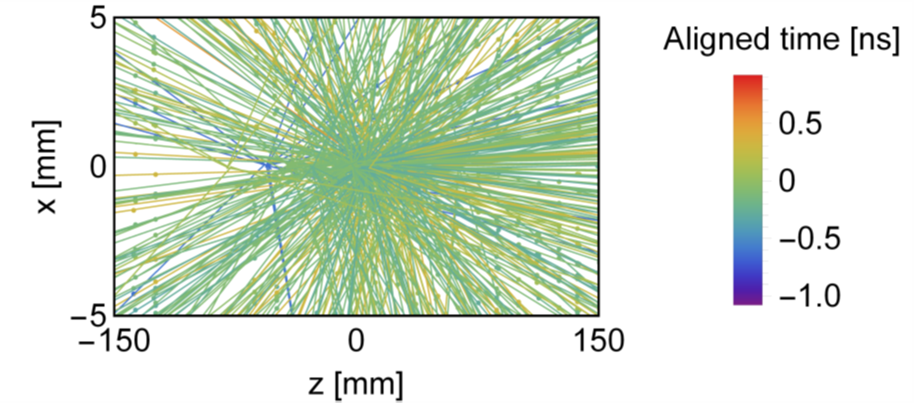
\includegraphics[width=1.0\linewidth]{TrackDensity1ns}
  \caption{time window = 1ns.}
  %\label{fig:sub1}
\end{subfigure}
\begin{subfigure}{.49\textwidth}
  \centering
  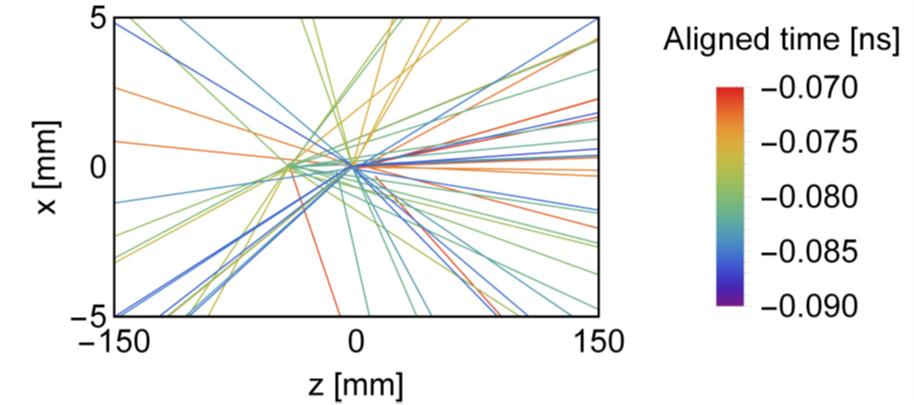
\includegraphics[width=1.0\linewidth]{TrackDensity20ps}
  \caption{time window = 20ps.}
  %\label{fig:sub2}
\end{subfigure}
\caption{Simulation of track density at VELO\cite{TDR}, generated by 42 collisions over one bunch crossing. Applying (b) a 20ps time cut to (a) the bunch crossing time period leaves only a few collisions and tracks. Among all LHCb subdetectors, VELO is the closest to the interaction point, and thus requires highest time resolution - see Fig. \ref{img:LHCbstructure}.}
\label{img:TrackDensity}
\end{figure}




%********************************** %Second Section  *************************************
\section{The LHCb Experiment}
\label{section2.2}

% Broad context of the LHCb
Up to the present time, there are nine experiments running at the LHC, each characterised by their detectors. The Large Hadron Collider beauty (LHCb) is the one that focuses on the study of the beauty quark (also known as the bottom quark) and aims to investigate the difference between matter and antimatter. 

In LHCb, data is collected from a series of subdetectors, each specialised to a slightly different function. These subdetectors stack behind each other layer-by-layer, and stretches over 20 metres from the collision point along the beam line. They are made to detect mainly the forward particles, as the beauty and charm hadrons and their decay products stay close to the beam line. This design makes LHCb a single forward-arm detector. 


\begin{figure}[h!]
\centering
\begin{subfigure}{.49\textwidth}
  \centering
  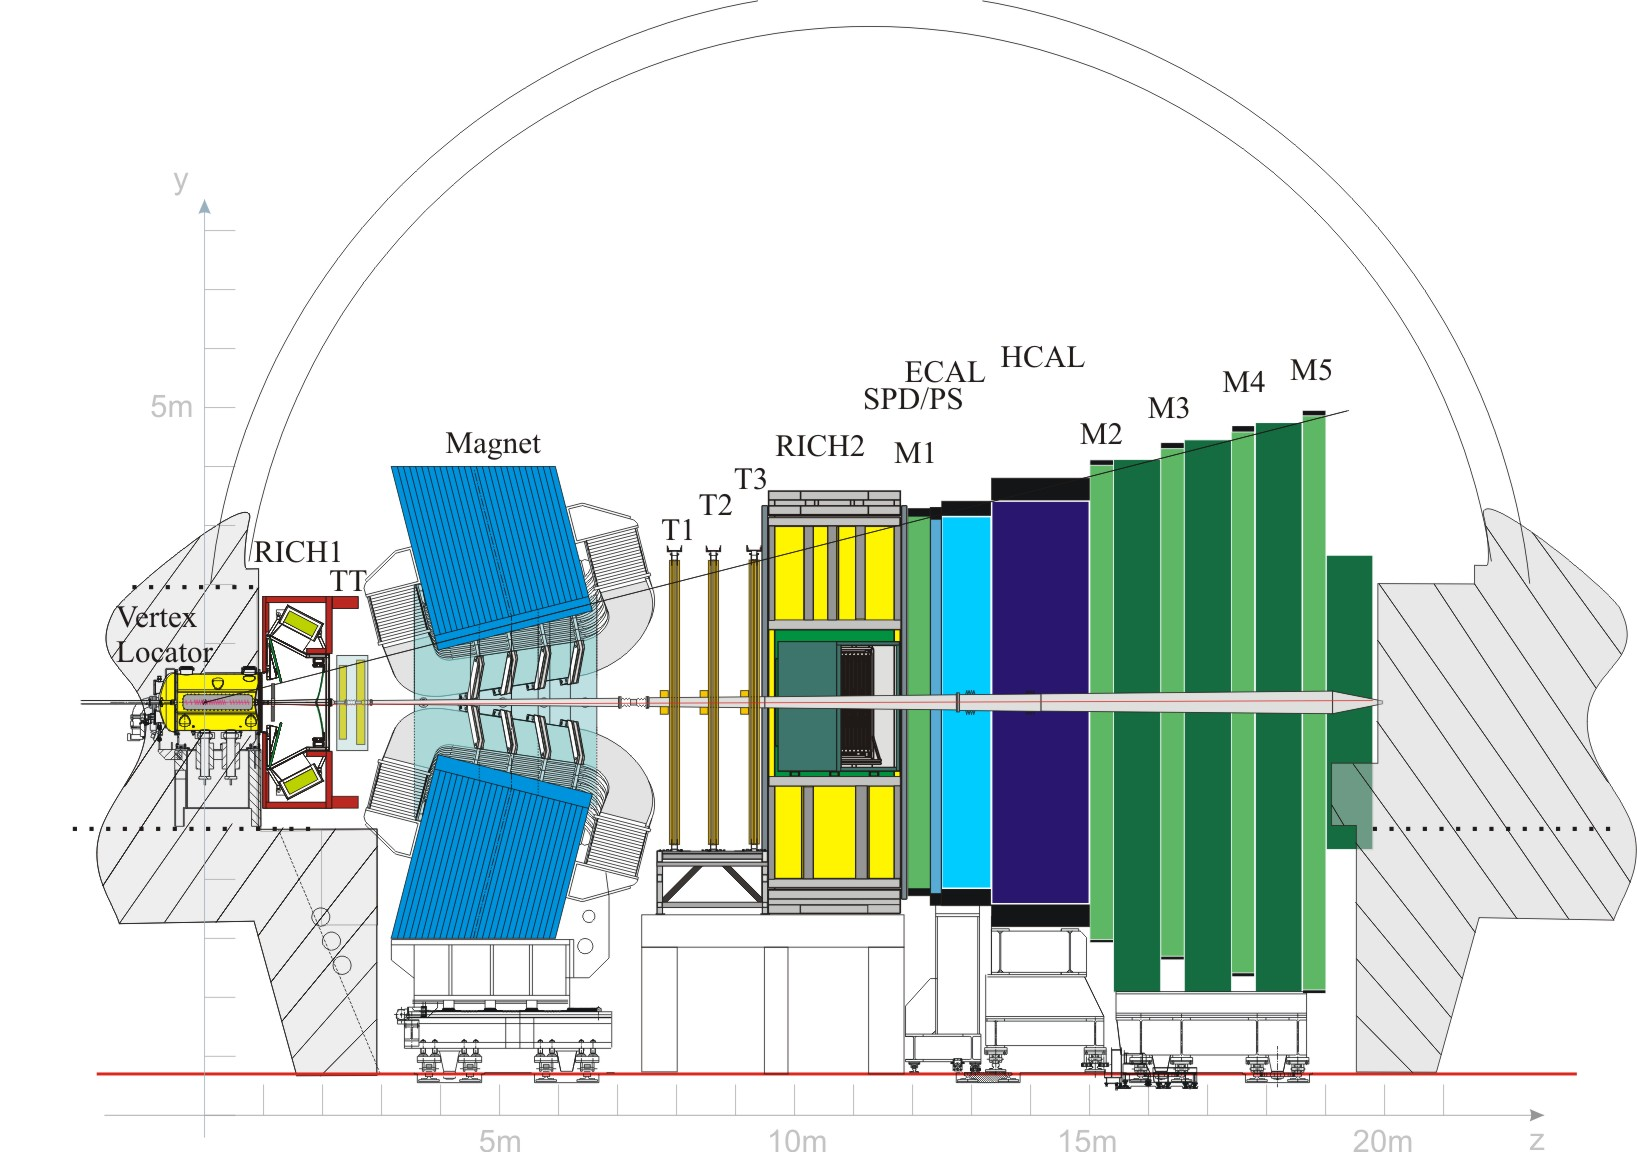
\includegraphics[width=1.0\linewidth]{LHCb}
  \caption{before Upgrade II.}
  %\label{fig:sub1}
\end{subfigure}
\begin{subfigure}{.49\textwidth}
  \centering
  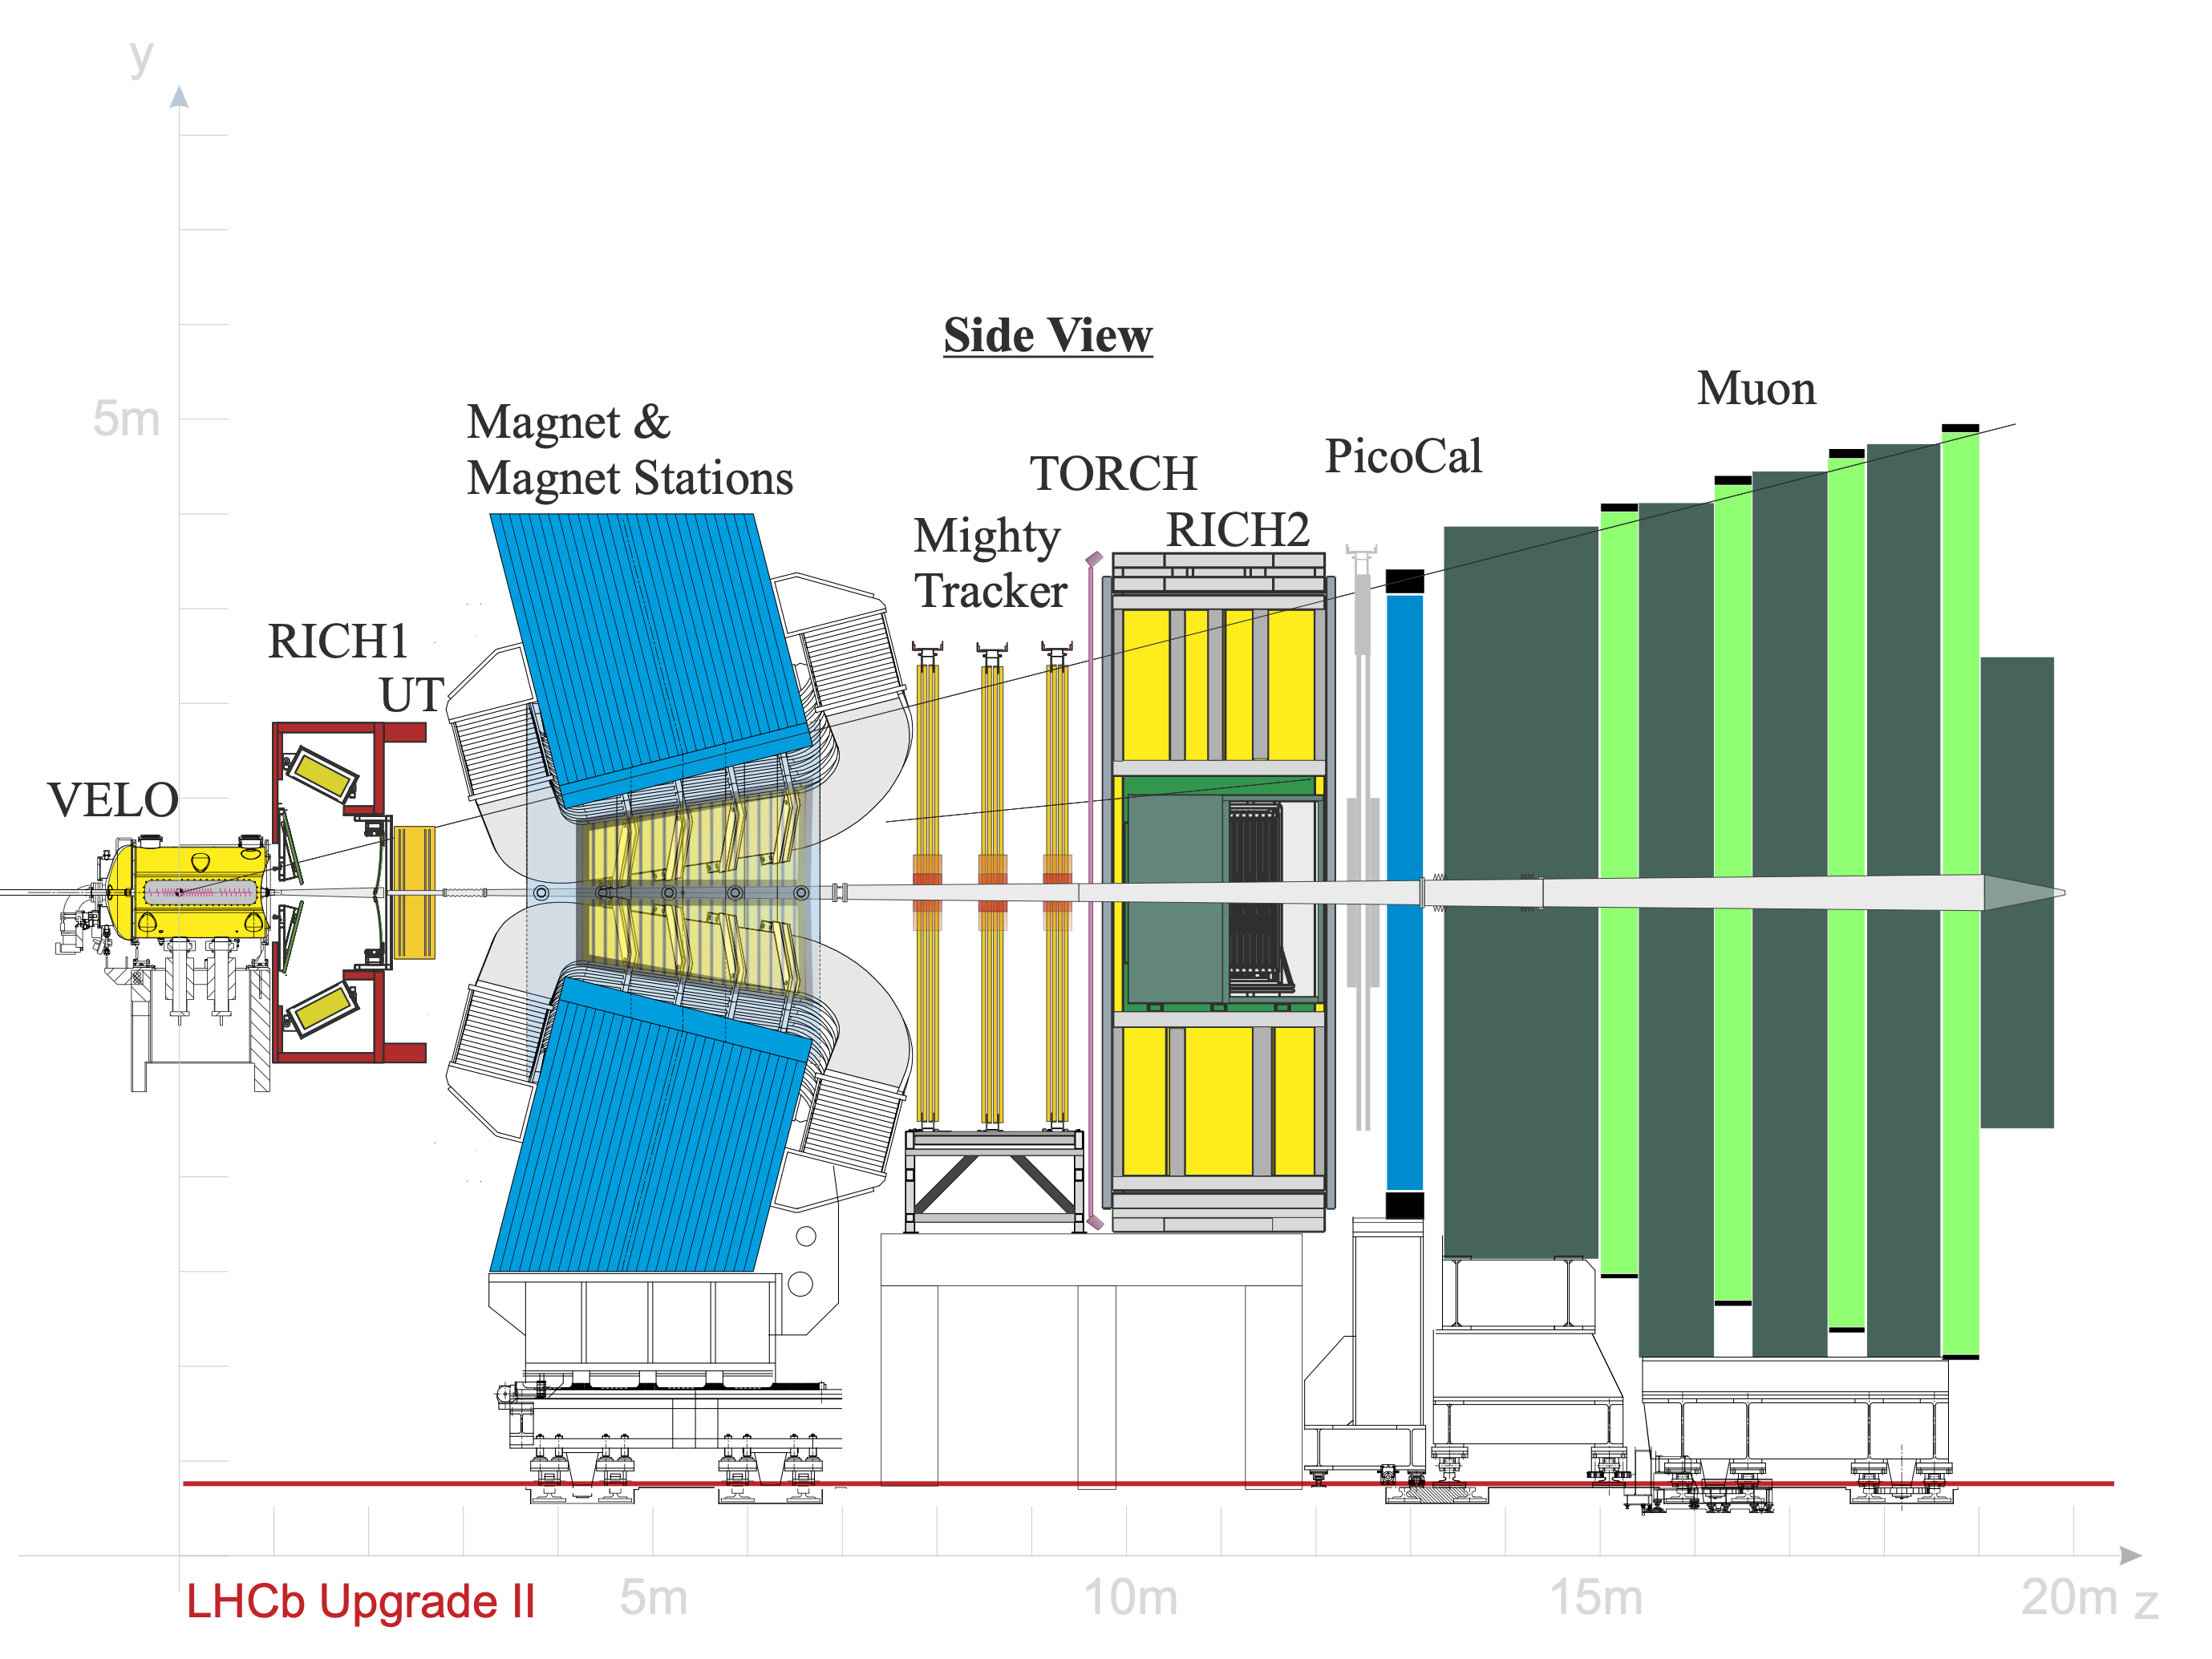
\includegraphics[width=1.0\linewidth]{LHCb_UgII}
  \caption{after Upgrade II.}
  %\label{fig:sub2}
\end{subfigure}
\caption{The structure of the LHCb spectrometer before and after Upgrade II\cite{TDR}. The subdetectors are labelled. During Upgrade II, the sensors will be upgraded, and magnet stations will be added to allow sensing in the magnet section.}
\label{img:LHCbstructure}
\end{figure}


% Talk about the changes to the detectors in Upgrade II
As a response to the higher-luminosity challenges from HL-LHC, the LHCb Upgrade II aims to improve the performance of the LHCb detector, allowing experiments to be performed under $7.5 \times$ higher pile-up value\cite{TDR}. This will be achieved by several methods, including the extensive use of MAPS technologies. The existing arrangement of the spectrometer and the majority of subdetectors will be kept, while certain components will be replaced. 



%********************************** % Third Section  *************************************
\section{The Mighty Tracker}  
\label{section2.3}

The MT is the fourth subdetector of the LHCb detector, as shown in Fig.\ref{img:LHCbstructure}. It consists of three tracking stations, each is divided into an outer and an inner tracker region. The outer region consists of four scintillating fibres (SciFi) detection planes, and each plane contains up to six modules of densely packed fibres. The inner region is equipped with two silicon panels, instrumented with high granularity silicon pixel sensors. A silicon panel is divided into 28 modules, each covers $20 \, cm \times 54 \, cm$. The beam passes through the centre of the tracking stations.

\begin{figure}[h!] 
\centering    
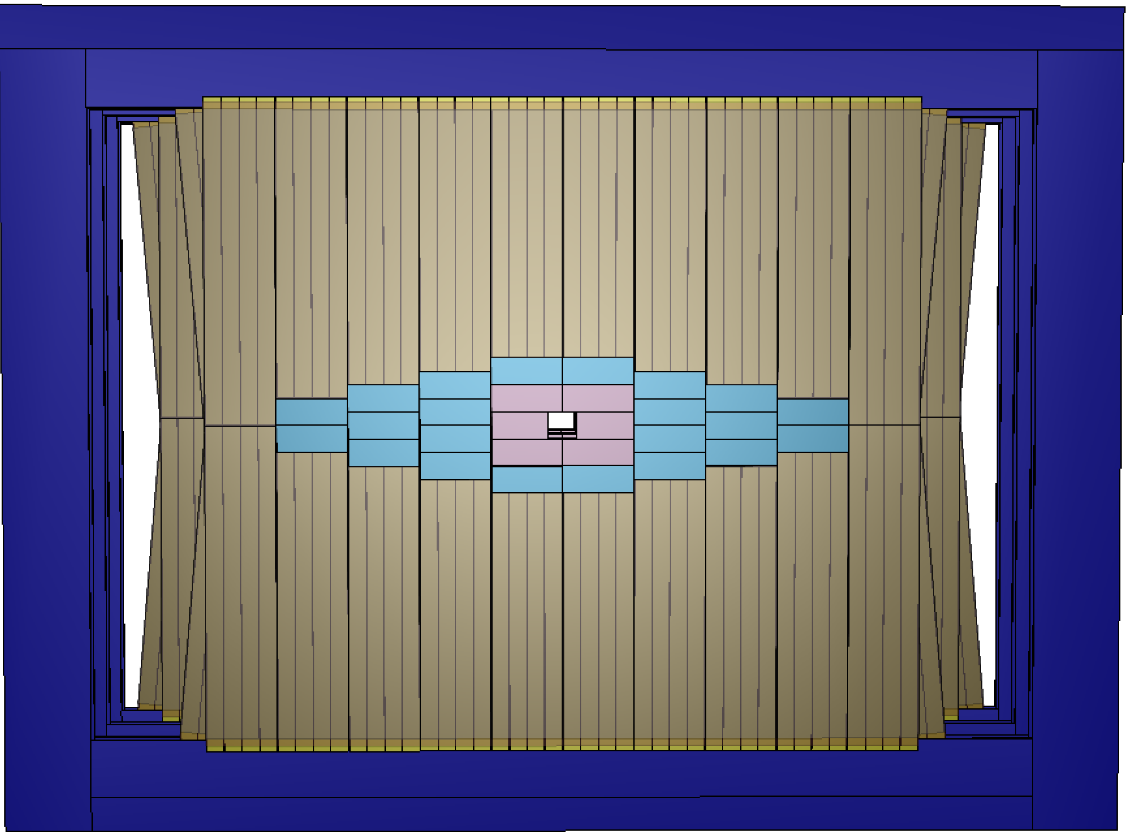
\includegraphics[width=0.6\linewidth]{MightyTracker}
\caption{The front view of the MT stations\cite{TDR}. The pink and light blue regions are covered with silicon sensors. The grey outer layer consists of 4 SciFi planes, two oriented vertically and two tilted by $\pm 5^\circ$ with respect to the vertical direction.}
\label{img:MightyTracker}
\end{figure}


% Discuss the requirements
%In the context of the Mighty Tracker, the recovery of pre-upgrade performance at higher luminosity requires:

%\begin{itemize}
%    \item Increase sensor granularity - distinguish between the primary vertices.
%    \item Minimise the rate of incorrect matching of upstream and downstream track segments.
%    \item Minimise material budget - reduce energy lost from travelling through the materials.
%    \item Exploit precision timing. 
    %【not entirely sure what this means】
%    \item Increase radiation hardness.
%\end{itemize}


%Under these requirements, 
To meet the requirement of recovering pre-upgrade performance, a mixed technology solution is adopted. For the central silicon pixel region, HV-MAPS produced by a commercial 180nm CMOS technology, are chosen for their radiation tolerance, capability of high-occupancy conditions, and lower costs compared to hybrid sensors. It has been widely used in all range of imaging-device applications, from low-end web-cams to high-end digital cameras\cite{HVMAPS}. For it to be used in scientific applications such as particle sensing, it must be tailored to meet the requirement of low noise, high speed, and radiation hardness. This will be discussed in details in Sec. \ref{section3.2}.

%For the scintillating fibres (SciFi), improved silicon photomultipliers (SiPM) are used for readout, with micro-lenses to improve light yield. The SciFi is kept at cryogenic temperature to reduce noise. 

With a bunch spacing of 25 ns\cite{HLLHC}, one bunch crossing is expected every 25 ns. Assuming a normal distribution of the hits, they need to be assigned correctly to the bunch crossing within 4$\sigma$, which means that 99.99\% of hits lies within 25 ns window. This requires a $\sigma<$3 ns, setting an requirement on sensor time resolution.
